%~~~~~~~~~~~~~~~~~~~~~~~~~~~~~~~~~~~~~~~~~~~~~~~~~~~~~~~~~~~~~~~~~~~~~
% Modelo de Teses e Dissertações CPAI: Textos ricos produzidos com Latex - v2012
% (v11)
%
%  Este modelo é trabalho de aperfeiçoamento de técnicas em Latex de:
%  Mamede Lima-Marques
%  Alfram Albuquerque
%  Alberto Magno Carvalho de Melo
%  Lauro César Araujo - laurocesar@laurocesar.com
%
%  Brasília, 19 de março de 2012
%
%~~~~~~~~~~~~~~~~~~~~~~~~~~~~~~~~~~~~~~~~~~~~~~~~~~~~~~~~~~~~~~~~~~~~~
                                                                                                                                                                                                                                                   
\documentclass[pnumplain,abnttoc,ruledheader,sumariocompleto,portuguese,twoside,openright]{report}
    
    % PACOTES GERAIS
    
    \usepackage[brazil]{babel}                 	% Determina os idiomas
	\usepackage[font=footnotesize,skip=4pt]{caption}[2011/11/10]	% captions
 	\usepackage{textcomp}						% Pacote de símbolos
 	\usepackage[T1]{fontenc}						% Seleção de códigos de fonte.
 	\usepackage{ucs}								% Usar Unicode
	\usepackage[utf8]{inputenc}					% Determina a codificação utiizada (conversão automática dos acentos)
	\usepackage[usenames,dvipsnames]{color}  	% Letras coloridas
	\usepackage{makeidx}                        % cria o indice
	\usepackage{constantes}						% pacote de constrantes
	\usepackage{teorema}                        % pacote com customizacoes deteorema 
	\usepackage{mathtools}   					% pacote matemático 
	\usepackage{dsfont}      					% matemático: simbolos de conjuntos 
	\usepackage{epigraph}    					% epigrafos no inicio dos capitulos
    \usepackage{bookmark,hyperref} 				% controlar a formação do índice
	\usepackage{multirow}						% Tabelas com células com múltiplas linhas
	\usepackage{longtable}						% Quebra de paginas em tabelas
	\usepackage{threeparttablex}					% notas no longtable
	\usepackage[nonumberlist,style=altlist]{glossaries}	% Glossario
		 			 			 		 				 		 				 			
	% PACOTES GRAFICOS
	
    \usepackage{float}							% permitir float nas figuras
    \ifx\pdfoutput\undefined
		% we are running LaTeX, not pdflatex
		\usepackage{graphicx}
	\else
		% we are running pdflatex, so convert .eps files to .pdf
		\usepackage[pdftex]{graphicx}
		\usepackage{epstopdf}
	\fi
	
	% PACOTES DE CITACOES
	
	\usepackage[brazilian,hyperpageref]{backref}	 % Paginas com as citações na bibl
	\usepackage{hyperref}						% Coloca links internos no arquivo
	\usepackage[alf]{abntcite}					% Citações padrão ABNT
	
	
	
	% Configurações do pacote backref
	\renewcommand{\backrefpagesname}				% Usado sem aopção hyperpageref de backref
		{Citado na(s) página(s): }
	\renewcommand{\backref}{}					% Texto padrão antes do número das páginas
	\renewcommand*{\backrefalt}[4]{				% Define os textos da citação
       \ifcase #1 %
         Nenhuma citação no texto.%
       \or
         Citado na página #2.%
       \else
         Citado #1 vezes nas páginas #2.%
		\fi 
	}
	
    % CONFIGURACOES DO PDF FINAL
    
     \hypersetup{
     	backref=true,
     	pagebackref=true,
		pdftitle={\meutitulo}, 
		pdfauthor={\autores - \autoresEmail},
		pdfkeywords={\palavrasChavesPortugues},
		bookmarks=true,         		% show bookmarks bar?
    		pdfsubject={\textoEpigrafe},
	    pdfproducer={Latex}, 	% producer of the document
    		colorlinks=true,       		% false: boxed links; true: colored links
    		linkcolor=blue,          	% color of internal links
    		citecolor=blue,        		% color of links to bibliography
    		filecolor=magenta,      		% color of file links
		urlcolor=blue,
		bookmarksdepth=4
		}


	% controla a pagina em branco deixada no lado par pelo twosides
	\makeatletter
	\def\cleardoublepage{
		\clearpage
		\if@twoside
			\ifodd %lado impar
				\c@page
			\else %lado par
				% imprimir texto centralizado
				\topskip0pt
				\vspace*{\fill}
					\begin{center}
						\textit{Esta página foi intencionalmente deixada em branco.}
					\end{center}
				\vspace*{\fill}
				
				% \hbox{}
	
				\thispagestyle{empty} 
				\newpage
				
				\if@twocolumn
					\hbox{}
					\newpage
				\fi
			\fi
		\fi
	}
	% \makeatothe

	% ----------------------------
	% CONTROLE DE MARGENS:
		
	% controla se as margens das páginas ímpares e pares
	% \oddsidemargin 0mm
	% \evensidemargin 0mm
	
	% controla outras margens	
	% \topmargin -10mm
	% \textwidth 16truecm
	% \textheight 24truecm
	% ----------------------------
				
	% PACOTES ADICIONAIS RECOMENDADOS:
	%\usepackage[brazil]{varioref}				% referencias ricas com \vref e \vpageref
	%\usepackage{collect}							% Coleta textos e permite reusá-los
				
				
%~~~~~~~~~~~~~~~~~~~~~~~~~~~~~~~~~~~~~~~~~~~~~~~~~~~~~~~~~~

%~~~~~~~~~~~~~~~~~~~~~~~~~~~~~~~~~~~~~~~~~~~~~~~~~~~~~~~~~~~~~~~~~~~~~
% INDICE REMISSIVO
%~~~~~~~~~~~~~~~~~~~~~~~~~~~~~~~~~~~~~~~~~~~~~~~~~~~~~~~~~~~~~~~~~~~~~

%índice
\makeindex

%~~~~~~~~~~~~~~~~~~~~~~~~~~~~~~~~~~~~~~~~~~~~~~~~~~~~~~~~~~~~~~~~~~~~~
% GLOSSÁRIO
%~~~~~~~~~~~~~~~~~~~~~~~~~~~~~~~~~~~~~~~~~~~~~~~~~~~~~~~~~~~~~~~~~~~~~

% Define a new glossary type
%\newglossary{main}{gls}{glo}{Glossário}
\makeglossaries

%~~~~~~~~~~~~~~~~~~~~~~~~~~~~~~~~~~~~~~~~~~~~~~~~~~~~~~~~~~~~~~~~~~~~~
%	MUDANÇA DE FONTES  
%	dos Capitulos e Seções para se adequar a norma ABNT
%~~~~~~~~~~~~~~~~~~~~~~~~~~~~~~~~~~~~~~~~~~~~~~~~~~~~~~~~~~~~~~~~~~~~~

%packages from abntex
%predefined abbreviations
\RequirePackage{abntex-default-design} 

% multicol - better multicolunms
\RequirePackage{multicol}

% ifthen - conditions in LaTeX
\RequirePackage{ifthen}

% calc - standard package for length and number easy calculations
\RequirePackage{calc}

%TODO INSERIR COMENTARIO INGLES
\RequirePackage{setspace}
%%%%%%%%%%%%%      OPTION DECLARATION      %%%%%%%%%%%%

%% Page numbering scheme
\providecommand{\ABNTpnum}{}
\DeclareOption{pagestart=folhaderosto} {\renewcommand{\ABNTpnum}{ABNT}}
\DeclareOption{pagestart=sumario}      {\renewcommand{\ABNTpnum}{plain}}
\DeclareOption{pagestart=firstchapter} {\renewcommand{\ABNTpnum}{RomSumArab}}
%deprecated options
\DeclareOption{pnumabnt}        {\ExecuteOptions{pagestart=folhaderosto}}
\DeclareOption{pnumplain}       {\ExecuteOptions{pagestart=sumario}}
\DeclareOption{pnumromarab}     {\ExecuteOptions{pagestart=firstchapter}}

%% Automatically include in TOC bibliography, index and stared chapters
\newboolean{ABNTincludeintoc}
\DeclareOption{sumario=completo}   {\setboolean{ABNTincludeintoc}{true}}
\DeclareOption{sumario=incompleto} {\setboolean{ABNTincludeintoc}{false}}
%deprecated options
\DeclareOption{sumariocompleto}    {\ExecuteOptions{sumario=completo}}
\DeclareOption{sumarioincompleto}  {\ExecuteOptions{sumario=incompleto}}

%% Style of page numbers in TOC
\newboolean{ABNTpagenumstyle}
\DeclareOption{tocpage=prefix} {\setboolean{ABNTpagenumstyle}{true}}
\DeclareOption{tocpage=plain}  {\setboolean{ABNTpagenumstyle}{false}}
%deprecated options
\DeclareOption{abnttoc}      {\ExecuteOptions{tocpage=prefix}}
\DeclareOption{normaltoc}    {\ExecuteOptions{tocpage=plain}}

%% Figures and tables independent of sections?

\newboolean{ABNTfigtabnumbers}
\DeclareOption{floatnumber=continuous} {\setboolean{ABNTfigtabnumbers}{true}}
\DeclareOption{floatnumber=chapter}    {\setboolean{ABNTfigtabnumbers}{false}}
%deprecated options
\DeclareOption{normalfigtabnum} {\ExecuteOptions{floatnumber=chapter}}
\DeclareOption{abntfigtabnum}   {\ExecuteOptions{floatnumber=continuous}}

%% Option: page headers
\newboolean{ABNTheader}
\providecommand{\ABNTheadertype}{\relax}
\DeclareOption{header=no}      {\setboolean{ABNTheader}{false}}
\DeclareOption{header=yes}     {\setboolean{ABNTheader}{true}}
\DeclareOption{header=normal}  {\ExecuteOptions{header=yes}\renewcommand{\ABNTheadertype}{normal}}
\DeclareOption{header=plain}   {\ExecuteOptions{header=yes}\renewcommand{\ABNTheadertype}{plain}}
\DeclareOption{header=ruled}   {\ExecuteOptions{header=yes}\renewcommand{\ABNTheadertype}{ruled}}
%%deprecated options
\DeclareOption{noheader}    {\ExecuteOptions{header=none}}
\DeclareOption{header}      {\ExecuteOptions{header=normal}}
\DeclareOption{plainheader} {\ExecuteOptions{header=plain}}
\DeclareOption{ruledheader} {\ExecuteOptions{header=ruled}}

%% Option `capchap', `capsec': 
%%   titles of chapters or sections in capital letters 
\newboolean{ABNTcapchap}              %true=titles of chapter/appendix in uppercase
\newboolean{ABNTcapsec}               %true=titles of sections in uppercase
\newboolean{ABNTCapAnnexAppendix}     %true=appendixname in uppercase
\newboolean{ABNTAnApName}             %true=show appendixname
\newboolean{ABNTAnApIndicativoIndent} %true=typeset title in a vbox

\ExecuteOptions{anapindicindent}
\DeclareOption{appendix=noname}     {\setboolean{ABNTAnApName}{false}}
\DeclareOption{appendix=Name}       {\setboolean{ABNTCapAnnexAppendix}{false}\setboolean{ABNTAnApName}{true}}
\DeclareOption{appendix=NAME}       {\setboolean{ABNTCapAnnexAppendix}{true}\setboolean{ABNTAnApName}{true}}
\DeclareOption{appendix=titlebox}   {\setboolean{ABNTAnApIndicativoIndent}{true}}
\DeclareOption{appendix=notitlebox} {\setboolean{ABNTAnApIndicativoIndent}{false}}
\DeclareOption{chapter=TITLE}       {\setboolean{ABNTcapchap}{true}\ExecuteOptions{appendix=NAME}}
\DeclareOption{chapter=Title}       {\setboolean{ABNTcapchap}{false}}
\DeclareOption{section=TITLE}       {\setboolean{ABNTcapsec}{true}}
\DeclareOption{section=Title}       {\setboolean{ABNTcapsec}{false}}
%%deprecated options
\DeclareOption{capchap}         {\ExecuteOptions{chapter=TITLE,appendix=NAME}}
\DeclareOption{capsec}          {\ExecuteOptions{section=TITLE}}
\DeclareOption{anapmaiusc}      {\ExecuteOptions{appendix=TITLE}}
\DeclareOption{anapnormal}      {\ExecuteOptions{appendix=Title}}
\DeclareOption{anapname}        {\ExecuteOptions{appendix=Name}}
\DeclareOption{anapnoname}      {\ExecuteOptions{appendix=noname}}
\DeclareOption{anapindicindent} {\ExecuteOptions{appendix=titlebox}}
\DeclareOption{anapcustomindent}{\ExecuteOptions{appendix=notitlebox}}

%% Line Spacing options: change current setting.
\newcommand*{\ABNTespacodefault}{} %
\DeclareOption{espaco=umemeio} {\renewcommand*{\ABNTespacodefault}{\taxaespacoumemeio}} % default
\DeclareOption{espaco=simples} {\renewcommand*{\ABNTespacodefault}{\taxaespacosimples}}
\DeclareOption{espaco=duplo}   {\renewcommand*{\ABNTespacodefault}{\taxaespacoduplo}}
%deprecated options
\DeclareOption{espacoumemeio} {\ExecuteOptions{espaco=umemeio}}
\DeclareOption{espacosimples} {\ExecuteOptions{espaco=simples}}
\DeclareOption{espacoduplo}   {\ExecuteOptions{espaco=duplo}}

%% Margin care --> Removed since version 1 beta

%% Options `spacednotes': removed since version 0.3
%  Assuming notes single spaced always (no alternative if using setspace ;-D

%% Auto bold math: bold math version ir text font is in bold face
\newboolean{ABNTautobm}
\DeclareOption{boldmath=auto}   {\setboolean{ABNTautobm}{true}}
\DeclareOption{boldmath=noauto} {\setboolean{ABNTautobm}{false}}
%deprecated options
\DeclareOption{autobm}   {\ExecuteOptions{boldmath=auto}}
\DeclareOption{noautobm} {\ExecuteOptions{boldmath=noauto}}

%% font option: times as default or not
\newboolean{ABNTtimesfont}
\DeclareOption{font=times}   {\setboolean{ABNTtimesfont}{true}}
\DeclareOption{font=plain}   {\setboolean{ABNTtimesfont}{false}}
%
\DeclareOption{times}   {\ExecuteOptions{font=times}}
\DeclareOption{notimes} {\ExecuteOptions{font=plain}}

%% Option to indent the first paragraph of each section or chapter
\newboolean{ABNTindentfirst}
\DeclareOption{indent=all}       {\setboolean{ABNTindentfirst}{true}}
\DeclareOption{indent=firstonly} {\setboolean{ABNTindentfirst}{false}}
%deprecated options
\DeclareOption{indentfirst}   {\ExecuteOptions{indent=all}}
\DeclareOption{noindentfirst} {\ExecuteOptions{indent=firstonly}}

%Options which group options according to specific norms.

%TODO AJUSTAR\DeclareOption{nbr6027=1989}  {\ExecuteOptions{tocpage=prefix}}
%TODO AJUSTAR \DeclareOption{nbr14724=2001} {%% $Id: nbr14724-2001.def,v 1.1 2004/07/12 09:47:55 gweber Exp $
%% name of this file nbr14724-2001.def
%% Copyright 2004 by the abnTeX group at http://abntex.codigolivre.org.br
%%
%% This file is distributed under the LaTeX-Project Public License (LPPL)
%%            http://www.latex-project.org/lppl.html
%% You are free to modify this file under the LPPL.
%%
%% $Log: nbr14724-2001.def,v $
%% Revision 1.1  2004/07/12 09:47:55  gweber
%% new definition file
%%

%clearly required
\ExecuteOptions{pagestart=folhaderosto}
\ExecuteOptions{sumario=completo}
\ExecuteOptions{tocpage=prefix}
\ExecuteOptions{floatnumber=continous}
\ExecuteOptions{header=plain}
\ExecuteOptions{chapter=Title,section=Title,appendix=NAME,appendix=titlebox,}
\ExecuteOptions{espaco=umemeio}
%our interpretation/understanding
\ExecuteOptions{appendix=titlebox,appendix=NAME}
\ExecuteOptions{indent=all}}
  
%options which declare version specific behaviour,
%default options expected for each version are declared here

\DeclareOption{abntex=0.8} 
  {\ExecuteOptions{boldmath=auto}
   \ExecuteOptions{font=times}
   \ExecuteOptions{nbr6027=1989,nbr14724=2001}
   \renewcommand{\ABNTbibliographyname}{\refname}}

\DeclareOption{abntex=0.9} 
  {\ExecuteOptions{boldmath=auto}
   \ExecuteOptions{font=times}
   \ExecuteOptions{nbr6027=1989,nbr14724=2001}}

% This should be the only default \ExecuteOptions command.
\ExecuteOptions{abntex=0.9}

\def\ABNTcurrentoptions{}
\newcommand{\AddCurrentOptionToList}{%
  \ifx\ABNTcurrentoptions\@empty%
     \edef\ABNTcurrentoptions{\CurrentOption}%
  \else%
     \edef\ABNTcurrentoptions{\ABNTcurrentoptions,\CurrentOption}%
  \fi%
}

%% All options not defined are passed to `report'
\DeclareOption*{%
  \AddCurrentOptionToList
% if some font or paper option is passed, a flag is set.
  \ifthenelse{\equal{\CurrentOption}{10pt}\or\equal{\CurrentOption}{11pt}}%
    {\setboolean{ABNTfontsize}{true}}{}%
  \ifthenelse{\equal{\CurrentOption}{a5paper}\or%
              \equal{\CurrentOption}{b5paper}\or%
              \equal{\CurrentOption}{letterpaper}}%
    {\setboolean{ABNTpaper}{true}}{}%
  \ifthenelse{\equal{\CurrentOption}{openany}}%
    {\setboolean{ABNTopen}{true}}{}%
  \PassOptionsToClass{\CurrentOption}{report}}


% testing if user use other options for font size or paper
% than 12pt, a4paper and openright
\newboolean{ABNTfontsize}
\setboolean{ABNTfontsize}{false}
\newboolean{ABNTpaper}
\setboolean{ABNTpaper}{false}
\newboolean{ABNTopen}
\setboolean{ABNTopen}{false}

% Process options (without star -> in the order of definition!).
\ProcessOptions
\newboolean{ABNThypertoc}
\newboolean{ABNTcapchap} 
\newboolean{ABNTheader}
\newcommand*{\taxaespacosimples}{1.}
\newcommand*{\taxaespacoumemeio}{1.35}
\newcommand*{\taxaespacoduplo}{1.7}

%%%%%%%%%%%%%%%%%%%%%%%%%%%%%%%%%%%%%%%%%%%%%%%%%%%%%%%%%%%%%%%%%%%%%
%  Line spacing stuff
%%%%%%%%%%%%%%%%%%%%%%%%%%%%%%%%%%%%%%%%%%%%%%%%%%%%%%%%%%%%%%%%%%%%%

% Since version 0.3 the `setspace' package is used.

% Space scheme in notes (footnotes and margin notes) removed since
% version 0.3 since setspace do not support it; footnotes are always
% single spaced!

% \espaco{} - ativa o espacamento para um numero dado (taxa de
% esticamento), mas aceita os parametros simples, umemeio, e duplo.

\newcommand{\espaco}[1]%
{\ifthenelse{\equal{#1}{simples}}% se espacamentos simples
  {\setstretch{\taxaespacosimples}} % entao
  { %senao (espaco simples)
   \ifthenelse{\equal{#1}{umemeio}}% se espaco 1 1/2
     {\setstretch{\taxaespacoumemeio}} % entao
     {%senao (espaco 1 1/2)
      \ifthenelse{\equal{#1}{duplo}}% se espaco duplo
        {\setstretch{\taxaespacoduplo}}% entao
        {\setstretch{#1}} % senao espaco dado
     } %fim se espaco 1 1/2
  } %fim se espaco simples
}%fim newcommand
\newenvironment{espacosimples}
  {\begin{spacing}{\taxaespacosimples}}{\end{spacing}}

\newenvironment{espacoumemeio}
  {\begin{spacing}{\taxaespacoumemeio}}{\end{spacing}}

\newenvironment{espacoduplo}%
  {\begin{spacing}{\taxaespacoduplo}}{\end{spacing}}
% After process options, flags are properly set.
% Passing options to class, that will be loaded in \LoadClass
\ifthenelse{\boolean{ABNTfontsize}}%
  {}{\PassOptionsToClass{12pt}{report}}
\ifthenelse{\boolean{ABNTpaper}}%
  {}{\PassOptionsToClass{a4paper}{report}}
\ifthenelse{\boolean{ABNTopen}}%
  {}{\PassOptionsToClass{openright}{report}}
  
  
\ifthenelse{\boolean{ABNTtimesfont}}% if `times'option enabled...
 {\IfFileExists{mathptmx.sty}%  try `mathptmx' first
    {\RequirePackage{mathptmx}}% 
    {\IfFileExists{mathptm.sty}% if not installed, try `mathptm'
       {\RequirePackage{mathptm}}%
       {\IfFileExists{times.sty} % 
         {\RequirePackage{times}}%
         {\renewcommand{\rmdefault}{ptm}}%
       }%
    }%
  \IfFileExists{helvet.sty}% including also Helvetica as sans serif.
    {\RequirePackage{helvet}}%
    {\IfFileExists{helvetic.sty}%
       {\RequirePackage{helvetic}}%
       {\renewcommand{\rmdefault}{phv}}%
    }%
 }%
 {}
 
 %%%%%%%%%%%%%%%%%%%%%%%%%%%%%%%%%%%%%%%%%%%%%%%%%%%%%%%%%%%%%%%%%%%%%%
%%    Setting margins
%%       (old Margin care mechanism removed since version 1 beta.)
%%%%%%%%%%%%%%%%%%%%%%%%%%%%%%%%%%%%%%%%%%%%%%%%%%%%%%%%%%%%%%%%%%%%%%

\ifthenelse{\boolean{ABNTheader}}%
  {%
   %%%%   VERTICAL LENGHTS  %%%%
   % The distance beetwen the top of the header and the top of the text is
   % of 1cm, this is,  1cm=\headheight+\headsep
   % ...but, we have to consider the depth of the header, addin 2mm.
   \setlength{\headsep}{1.2cm-\headheight}
   % The distance beetwen the paper border and the number must be 2cm
   % 2cm=\topmargin+\voffset+1in
    \setlength{\topmargin}{2cm-1in-\voffset} 
   % The inferior border must be 2cm
   % \paperheight=\topmargin+\voffset+1in+\headheight+\headsep+\textheight+2cm
    \setlength{\textheight}% 
      {\paperheight-\topmargin-\voffset-1in-\headheight-\headsep-2cm}
  }%
  {% no header is not ABNT!!!
   % Let's fake it: 2cm each vertical margin and de same horizontal margin.
   \setlength{\topmargin}{2cm-\headheight-\headsep-\voffset-1in}
   \setlength{\textheight}% 
      {\paperheight-2cm-\footskip-2cm}
  }%

%%%%   HORIZONTAL LENGHTS   %%%%
% The left margin is 3cm, and the right margin equals to 2cm.
\setlength{\oddsidemargin}{3cm-\hoffset-1in}
% for compatibility with twoside print, the length of the margins must
% be exchanged.
\setlength{\evensidemargin}{2cm-\hoffset-1in}
% \paperwidth=\textwidth+\oddsidemargin+\hoffset+1in+2cm
\setlength{\textwidth}{\paperwidth-\oddsidemargin-\hoffset-1in-2cm}
 
 %%%%% auto bold math (try follow bold face in text)

% plan: redefine commands that change font to bold to ALSO change math
% version; I don't change all commands that change font weight because I
% suppose this uses are local

\AtBeginDocument{
\ifthenelse{\boolean{ABNTautobm}\and\not\isundefined{\mv@bold}}%
 {%
  % \bfseries
  \let\ABNToldbfseries\bfseries\relax%
  \renewcommand{\bfseries}{\mathversion{bold}\ABNToldbfseries}%
  %
  % \textbf{}
  \let\ABNToldtextbf\textbf\relax%
  \renewcommand{\textbf}[1]{\ABNToldtextbf{\mathversion{bold}#1}}%
  %
  % \bf
  \let\ABNToldbf\bf\relax%
  \renewcommand{\bf}{\mathversion{bold}\ABNToldbf}%
  %
 }%
 {}%
}

%%%%%%    Indent code 

% indenting first paragraph of each section
\ifthenelse{\boolean{ABNTindentfirst}}%
 {\RequirePackage{indentfirst}}%
 {}

% paragraph indentation size and skip
\setlength{\parindent}{.7cm}
\setlength{\parskip}{.25cm}
 
%%%%%%%%%%%%%%%%%%%%%%%%%%%%%%%%%%%%%%%%%%%%%%%%%%%%%%
%    Page styles available: 
%         plainheader, header, ruledheader
%%%%%%%%%%%%%%%%%%%%%%%%%%%%%%%%%%%%%%%%%%%%%%%%%%%%%%

\newcommand{\ABNTmarkboth}[2]{%
 \ifthenelse{\boolean{ABNTNextOutOfTOC}}
     {\markboth{\ABNTnextmark}{\ABNTnextmark}}
     {\markboth{#1}{#2}}%
 }

\newcommand{\ABNTmarkright}[1]{%
 \ifthenelse{\boolean{ABNTNextOutOfTOC}}
     {\markright{\ABNTnextmark}}
     {\markright{#1}}%
 }


%%%%%%%  Defining pagestyle "header"
%
\newcommand{\ps@header}{%
  \renewcommand{\@oddfoot}{}%
  \renewcommand{\@evenfoot}{}%
  \renewcommand{\@oddhead}%
    {{\rightmarkformat\rightmark}\hfill{\thepageformat\thepage}}%
  \renewcommand{\@evenhead}%
       {{\thepageformat\thepage}\hfill{\leftmarkformat\leftmark}}%
% Para \chapter* mostrar o cabecalho
  \let\@mkboth\ABNTmarkboth%
% Definindo a maneira como o comando o \chapter marca o cabecalho
  \renewcommand{\chaptermark}[1]{%
    \markboth%
       {\ifnum \c@secnumdepth >\m@ne%
            \thechapter{}  %
        \fi%
        ##1}%
       {\ifnum \c@secnumdepth >\m@ne%
            \thechapter{}  %
        \fi%
        ##1}%
  }%
  \renewcommand{\sectionmark}[1]{%
    \markright{%
      \ifnum \c@secnumdepth >\z@%
        \thesection\ \ %
      \fi%
      ##1}%
  }%   
}% 
 %%  Defining pagestyle plainheader
%
\newcommand{\ps@plainheader}{%
  \renewcommand{\@oddfoot}{}%
  \renewcommand{\@evenfoot}{}%
  \renewcommand{\@oddhead}{\hfill{\thepageformat\thepage}}%
  \renewcommand{\@evenhead}{{\thepageformat\thepage}\hfill}%
% Para \chapter* mostrar o cabecalho
  \let\@mkboth\ABNTmarkboth%
% Definindo a maneira como o comando o \chapter marca o cabecalho
  \renewcommand{\chaptermark}[1]{%
    \markboth%
       {\ifnum \c@secnumdepth >\m@ne%
            \thechapter\ \ %
        \fi%
        ##1}%
       {\ifnum \c@secnumdepth >\m@ne%
            \thechapter\ \ %
        \fi%
        ##1}%
  }%
  \renewcommand{\sectionmark}[1]{%
    \markright{%
      \ifnum \c@secnumdepth >\z@%
        \thesection\ \ %
      \fi%
      ##1}%
  }%   
}% 
 %%  Defining pagestyle ruledheader
%
\newcommand{\ps@ruledheader}{%
  \renewcommand{\@oddfoot}{}%
  \renewcommand{\@evenfoot}{}%
  \renewcommand{\@oddhead}%
     {\underline{\makebox[\textwidth]{\raisebox{-.5ex}{}%
       {\rightmarkformat\rightmark}\hfill{\thepageformat\thepage}}}}%
  \renewcommand{\@evenhead}%
     {\underline{\makebox[\textwidth]{\raisebox{-.5ex}{}%
       {\thepageformat\thepage}\hfill{\leftmarkformat\leftmark}}}}%
% Para \chapter* mostrar o cabecalho
  \let\@mkboth\ABNTmarkboth%
% Definindo a maneira como o comando o \chapter marca o cabecalho
  \renewcommand{\chaptermark}[1]{%
    \markboth%
       {\ifnum \c@secnumdepth >\m@ne%
            \thechapter\ \ %
        \fi%
        ##1}%
       {\ifnum \c@secnumdepth >\m@ne%
            \thechapter\ \ %
        \fi%
        ##1}%
  }%
  \renewcommand{\sectionmark}[1]{%
    \markright{%
      \ifnum \c@secnumdepth >\z@%
        \thesection\ \ %
      \fi%
      ##1}%
  }%   
}% 
%%%%%%%%%%%%%%%%%%%%%%%%%%%%%%%%%%%%%%%%%%%%%%%%%%%%%%%%%%%%%%%%%%%%%%%
%%    Page numbering 
%%%%%%%%%%%%%%%%%%%%%%%%%%%%%%%%%%%%%%%%%%%%%%%%%%%%%%%%%%%%%%%%%%%%%%%

\newboolean{ABNTinpretext}
\setboolean{ABNTinpretext}{true}

\newboolean{ABNTaftertoc}
\setboolean{ABNTaftertoc}{false}

% The command \ABNTBeginOfTextualPart is executed by \tableofcontents at
% its end. It's intented to page style and page number settings.
\providecommand{\ABNTBeginOfTextualPart}{}

\newcommand{\chaptertitlepagestyle}{plain}

\ifthenelse{\equal{\ABNTpnum}{plain}}
  {%
    \setboolean{ABNTinpretext}{false}
    \setboolean{ABNTaftertoc}{true}
    \ifthenelse{\boolean{ABNTheader}}
       {%
        \ifthenelse{\equal{\ABNTheadertype}{plain}}%
          {\pagestyle{plainheader}}
          {%
           \ifthenelse{\equal{\ABNTheadertype}{normal}}%
             {\pagestyle{header}}%
             {\pagestyle{ruledheader}}%
          }%
        \renewcommand{\chaptertitlepagestyle}{plainheader}%
       }%
       {%
        \pagestyle{plain}%
        \renewcommand{\chaptertitlepagestyle}{plain}
       }%
  }% 
  {%
   \ifthenelse{\equal{\ABNTpnum}{ABNT}}%
     {% ABNT strict
      % - pagestyle is empty until \tableofcontents, when it becames with
      %   numeration (depending on `header' or `plain' header style)
      % - page counter starts AT `folha de rosto'.
      %
      % Makeing titlepage environment increase page counter
      \let\ABNToldendtitlepage\endtitlepage\relax
      \renewcommand{\endtitlepage}{\ABNToldendtitlepage\addtocounter{page}{1}}
      \pagestyle{empty}
      \renewcommand{\thepage}{}
      \renewcommand{\chaptertitlepagestyle}{empty}
      \renewcommand{\ABNTBeginOfTextualPart}%
        {%
         \renewcommand{\thepage}{\arabic{page}}
         \ifthenelse{\boolean{ABNTheader}}
           {%
            \ifthenelse{\equal{\ABNTheadertype}{plain}}%
              {\pagestyle{plainheader}}
              {%
               \ifthenelse{\equal{\ABNTheadertype}{normal}}%
                 {\pagestyle{header}}%
                 {\pagestyle{ruledheader}}%
              }%
            \renewcommand{\chaptertitlepagestyle}{plainheader}%
           }%
           {%
            \pagestyle{plain}%
            \renewcommand{\chaptertitlepagestyle}{plain}
           }%

        }%
     }%
     {% RomArab
      % - page style with numeration 
      % - BEFORE \tableofcontents
      %     \thepage in roman
      %     page counter starts AFTER `folha de rosto'
      % - AFTER \tableofcontents
      %     \thepage in arabic
      %     page counter starts again
      %
      \ifthenelse{\boolean{ABNTheader}}
        {%
         \ifthenelse{\equal{\ABNTheadertype}{plain}}%
           {\pagestyle{plainheader}}
           {%
            \ifthenelse{\equal{\ABNTheadertype}{normal}}%
              {\pagestyle{header}}%
              {\pagestyle{ruledheader}}%
           }%
         \renewcommand{\chaptertitlepagestyle}{plainheader}%
        }%
        {%
         \pagestyle{plain}%
         \renewcommand{\chaptertitlepagestyle}{plain}
        }%
      \renewcommand{\thepage}{\roman{page}}
      \renewcommand{\ABNTBeginOfTextualPart}%
        {%
         \renewcommand{\thepage}{\arabic{page}}
         \setcounter{page}{1}
        }%
     }%
  }%
%%%%%%%%%%%%%%%%%%%%%%%%%%%%%%%%%%%%%%%%%%%%%%%%%%%%%%%%%%%%%%%%%%%%%
%%    Chapter title page style
%%%%%%%%%%%%%%%%%%%%%%%%%%%%%%%%%%%%%%%%%%%%%%%%%%%%%%%%%%%%%%%%%%%%%

% Redefining \chapter and \part. The changes are
%  - \chapteritlepagestyle instead of explict plain page style
%  - \ABNTchaptermark instead of \chaptermark (must be before
%       \addcontentsline !!!)
% - several commands were replaced by abntversions due to nuances of the
%   norms :-( it can create several uncompatibilities with packages that
%   change explictily these important commands, although I have tried very
%   hard to make as less damage on compatibility as possible. As a result
%   of this, package hyperref is totally broken with abnt.cls.

%%%%%%%%%%%%%%%%%%%%%%   Special definitions   %%%%%%%%%%%%%%%%%%%%
% What is going on here?
%   
%  This class supports auto include in toc for both \chapter* and
%  \section* (and similars). As we know, the command \chapter admits an
%  optional argument, which goes to the toc and the marks, if it's present
%  (otherwise the main parameter of \chapter is used in toc and marks also.)
%  
%  To allow exactly the same mechanism for \chapter and \chapter*, \section
%  and \section*, \subsection and \subsection*, etc, I had to define
%  similar commands to some important core commands in LaTeX, like \secdef
%  (we make a new one to avoid conflicts with other packages) and
%  \@startsection (I make a new one too).
%
%  Now, \ABNTstartsection, appart from make the stared version of a
%  section-like command to include the title in toc (if a boolean is set to
%  true), the title is centered for stared form.
%
%  Now, \chapter* and \part* are almost equal to \chapter and \part
%
%  The origin of this material are the files 
%     $texmfDIR/tex/latex/base/latex.ltx  (codigo fonte do LaTeX)
%     $texmfDIR/tex/latex/base/report.cls (classe standard)

% From the definition of \secdef -> stared version now admits optional
% param (after bug with hyperref, it was no longer used.)
\def\ABNTsecdef#1#2{\@ifstar{\@dblarg{#2}}{\@dblarg{#1}}}

% Changed explicit \thispagestyle{empty}


%chaptertype is necessary to correctly generate hyperref's targets
\newcommand{\chaptertype}{}%

\newcommand{\setchaptertype}[1]{\gdef\chaptertype{#1.}}
  
\renewcommand\chapter%
    {%
     \if@openright\cleardoublepage\else\clearpage\fi%
     \thispagestyle{\chaptertitlepagestyle}
     \ifthenelse{\boolean{ABNTinpretext}}%
       {%
        \ifthenelse{\boolean{ABNTaftertoc}}%
          {% change to textual part
           \setboolean{ABNTinpretext}{false}%
           \ABNTBeginOfTextualPart%
          }%
          {}%
       }% 
       {}%
     \global\@topnum\z@%
     \@afterindentfalse%
%     \ABNTsecdef\@chapter\@schapter%
    \secdef\@chapter\@schapter%
    }%

% To make pre-textual chapters (that fits page numbering squeme...)
% this is equal to \chapter*{}, but ignores in witch part is it. It does
% not change any tags.
\newcommand\pretextualchapter%
    {%
     \if@openright\cleardoublepage\else\clearpage\fi%
     \thispagestyle{\chaptertitlepagestyle}
     \global\@topnum\z@%
     \@afterindentfalse%
     \@schapter%
    }%

% Created useful \resetsubcounters from the code of \stepcounter.
\newcommand{\resetsubcounters}[1]{%
  \begingroup
    \let\@elt\@stpelt
    \csname cl@#1\endcsname
  \endgroup}

%% \ProximoForaDoSumario -> taking out some chapter or section from toc.

\newboolean{ABNTNextOutOfTOC}
\setboolean{ABNTNextOutOfTOC}{false}

%% \ProximoForaDoSumario[mark text]
% Now \ProximoForaDoSumario (re)sets the marks too. If one still want the
% marks, he/she must use it as the optional parameter of this command.

\newcommand{\ABNTnextmark}{}
\newcommand{\ProximoForaDoSumario}[1][]
  {
   \setboolean{ABNTNextOutOfTOC}{true}
   \renewcommand{\ABNTnextmark}{#1}
  }

\newcommand{\ABNTaddcontentsline}[3]
  {\ifthenelse{\boolean{ABNTNextOutOfTOC}}
     {\setboolean{ABNTNextOutOfTOC}{false}}
     {\addcontentsline{#1}{#2}{#3}}}

\newcommand{\ABNTchaptermark}[1]
  {%
   \ifthenelse{\boolean{ABNTNextOutOfTOC}}
     {\markboth{\ABNTnextmark}{\ABNTnextmark}}
     {\chaptermark{#1}}%
  }

\newcommand{\ABNTsectionmark}[1]
  {%
   \ifthenelse{\boolean{ABNTNextOutOfTOC}}
     {\markright{\ABNTnextmark}}
     {\sectionmark{#1}}%
  }


% \@chapter : 
\def\@chapter[#1]#2%
      {\ifthenelse{\boolean{ABNThypertoc}}{\renewcommand{\theHchapter}{\chaptertype\thechapter}}{}
       \ifnum \c@secnumdepth >\m@ne %report.cls
         \refstepcounter{chapter}   %report.cls
         \ABNTchaptermark{#1}% This command MUST come before addcontentsline
         \typeout{\@chapapp\space\thechapter.}%report.cls
         \ifthenelse{\boolean{ABNTaftertoc}}
           {\ABNTaddcontentsline{toc}{chapter}{\protect\numberline{\thechapter}#1}}%true
           {}%false
       \else%report.cls
         \ABNTchaptermark{#1}% This command MUST come before addcontentsline
         \ifthenelse{\boolean{ABNTaftertoc}}%
           {\ABNTaddcontentsline{toc}{chapter}{#1}}%true
           {}%false
       \fi%end of ifnum
       %%%begin report.cls
       \if@twocolumn
         \@topnewpage[\@makechapterhead{#2}]%
       \else
         \@makechapterhead{#2}%
         \@afterheading
       \fi
       \par}

%% From the \@chapter code. Now \@schapter does almost the same as
%% \@chapter. Added \resetsubcounters.
\def\@schapter#1{%
      \ifthenelse{\boolean{ABNThypertoc}}{\renewcommand{\theHchapter}{\chaptertype\thechapter}}{}
      \if@twocolumn
        \@topnewpage[\@makeschapterhead{#1}]
      \else
        \@makeschapterhead{#1}
        \@afterheading
      \fi
      \@mkboth{#1}{#1}  % <-- inserted (must be before addcontentsline)
      \ifthenelse{\boolean{ABNTincludeintoc}}%
        {%
         \ifthenelse{\boolean{ABNTaftertoc}}
           {\ABNTaddcontentsline{toc}{chapter}{#1}}
           {}
        }%
        {}
      \resetsubcounters{chapter}\par
    }%
%TODO VERIFICAR O CODIGO DE PART
% Fonts in \@part and \@part* changed. Some \resetsubcounters added.
\def\@part[#1]#2{%
    \ifnum \c@secnumdepth >-2\relax
      \refstepcounter{part}%
      \ABNTaddcontentsline{toc}{part}{\protect\numberline{\thepart}#1}%
    \else
      \resetsubcounters{part}
      \ABNTaddcontentsline{toc}{part}{#1}%
    \fi
    \markboth{}{}%
    {\centering
     \interlinepenalty \@M
     \normalfont
     \ifnum \c@secnumdepth >-2\relax
       \ABNTchapterfont\huge\ifthenelse{\boolean{ABNTcapchap}}%
          {\MakeUppercase{\partname~\thepart}}%
          {\partname~\thepart}
       \par
       \vskip 20\p@
     \fi
     \ABNTchapterfont\Huge\ifthenelse{\boolean{ABNTcapchap}}%
          {\MakeUppercase{#2}}%
          {#2}\par}%
    \@endpart}

\def\@spart#1{%
    \ABNTaddcontentsline{toc}{part}{#1}%
    \markboth{}{}%
    {\centering
     \interlinepenalty \@M
     \normalfont
     \ABNTchapterfont\Huge\ifthenelse{\boolean{ABNTcapchap}}%
          {\MakeUppercase{#1}}%
          {#1}\par}%
    \@endpart}
    
    
    
    
%TODO VERIFICAR ESSA CONFIGURACAO CAPITULO
%% Font which chapter titles will be printed
\ifthenelse{\boolean{ABNTcapchap}}
  {\newcommand{\ABNTchapterfont}{\ABNTCHAPTERfont}}%uppercase
  {\newcommand{\ABNTchapterfont}{\ABNTChapterfont}}%titlecase

%% In order to \MakeUppercase do not apply to math mode in chapter or
%% section titles, package textcase used
%
% Sorry, a bug on textcase adds extra space before text. User can fix it by
% him/herself.
%
%\ifthenelse{\boolean{ABNTcapchap}\or\boolean{ABNTcapsec}}
%  {\IfFileExists{textcase.sty}
%     {\RequirePackage[overload]{textcase}}
%     {}
%  }
%  {}

% Defining how is typeset the \chapter
\def\@makechapterhead#1{%
  {%
%  \noindent\rule{\textwidth}{1.7pt}\\\par
  \normalfont\ABNTchaptersize\ABNTchapterfont%
  \espaco{simples}%
  \vspace*{30pt}%
  \noindent%
  \parbox[b]{\textwidth}{%
    \parbox[t]{4ex}{\thechapter}%
    \parbox[t]{\textwidth-4ex-1ex}%
      {\interlinepenalty\@M\raggedright%
        \ifthenelse{\boolean{ABNTcapchap}}%
          {\MakeUppercase{#1}}%
          {#1}
      }%
    \vspace*{0cm}
    }\\[2pt]%
  \vspace{50pt}%
  }%
}

% Defining how is typeset the \chapter*
\def\@makeschapterhead#1{%
  \vspace*{0pt}\par
  {\centering\normalfont\ABNTchaptersize\ABNTchapterfont%
   \ifthenelse{\boolean{ABNTcapchap}}%
     {\MakeUppercase{#1}}%
     {#1}
    \par}%
  \vspace{45pt}%
  \par%
}

% redefining to apply tocnumpageabnt
\renewcommand\l@chapter[2]{%
  \ifnum \c@tocdepth >\m@ne
    \addpenalty{-\@highpenalty}%
    \vskip 1.0em \@plus\p@
    \setlength\@tempdima{1.5em}%
    \begingroup
      \ifthenelse{\boolean{ABNTpagenumstyle}}
        {\renewcommand{\@pnumwidth}{3.5em}}
        {}
      \parindent \z@ \rightskip \@pnumwidth
      \parfillskip -\@pnumwidth
      \leavevmode \normalsize\ABNTtocchapterfont
      \advance\leftskip\@tempdima
      \hskip -\leftskip
      #1\nobreak\hfil \nobreak%
      \ifthenelse{\boolean{ABNTpagenumstyle}}
         {%
          \hb@xt@\@pnumwidth{\hss 
            \ifthenelse{\not\equal{#2}{}}{{\normalfont p.\thinspace#2}}{}}\par
         }
         {%
          \hb@xt@\@pnumwidth{\hss #2}\par
         }
      \penalty\@highpenalty
    \endgroup
  \fi}    
% From \@startsection. The only difference is that it calls \@ssect
% changing the meaning id the first parameter. Now, instead of indentation,
% it gives section level for TOC purposes.
\def\ABNTstartsection#1#2#3#4#5#6{%
  \if@noskipsec \leavevmode \fi
  \par
  \@tempskipa #4\relax
  \@afterindenttrue
  \ifdim \@tempskipa <\z@
    \@tempskipa -\@tempskipa \@afterindentfalse
  \fi
  \if@nobreak
    \everypar{}%
  \else
    \addpenalty\@secpenalty\addvspace\@tempskipa
  \fi
  \@ifstar
    {\ABNTssect{#1}{#4}{#5}{#6}}% #3 replaced by #1 here
    {\@dblarg{\ABNTsect{#1}{#2}{#3}{#4}{#5}{#6}}}}

% I change the meaning of the first paramenter here. Instead of an indent
% skip, it is now the name of the section, for `toc' purposes.
\def\ABNTssect#1#2#3#4#5{%
  \@tempskipa #3\relax
  \ifdim \@tempskipa>\z@
    \begingroup
      #4{%
         \interlinepenalty \@M \centering
         \ifthenelse{\boolean{ABNTcapsec}}
             {\MakeUppercase{#5}}{#5}\@@par}%
    \endgroup
    \@ifundefined{ABNT#1mark}{}{\csname ABNT#1mark\endcsname{#5}}
    \ifthenelse{\boolean{ABNTincludeintoc}}
      {\ABNTaddcontentsline{toc}{#1}{#5}}
     {}
  \else
    \def\@svsechd{#4{#5}%
      \@ifundefined{ABNT#1mark}{}{\csname ABNT#1mark\endcsname{#5}}
      \ifthenelse{\boolean{ABNTincludeintoc}}%
         {\ABNTaddcontentsline{toc}{#1}{#5}}{}
    }%
  \fi
  \@xsect{#3}}

\def\ABNTsect#1#2#3#4#5#6[#7]#8{%
  \ifnum #2>\c@secnumdepth
    \let\@svsec\@empty
  \else
    \refstepcounter{#1}%
    \protected@edef\@svsec{\@seccntformat{#1}\relax}%
  \fi
  \@tempskipa #5\relax
  \ifdim \@tempskipa>\z@
    \begingroup
      #6{%
        \@hangfrom{\hskip #3\relax\@svsec}%
          \interlinepenalty \@M
          \ifthenelse{\boolean{ABNTcapsec}}
             {\MakeUppercase{#8}}{#8}\@@par}%
    \endgroup
    \@ifundefined{ABNT#1mark}{}{\csname ABNT#1mark\endcsname{#7}}
    \ABNTaddcontentsline{toc}{#1}{%
      \ifnum #2>\c@secnumdepth \else
        \protect\numberline{\csname the#1\endcsname}%
      \fi
      #7}%
  \else
    \def\@svsechd{%
      #6{\hskip #3\relax
      \@svsec \ifthenelse{\boolean{ABNTcapsec}}
             {\MakeUppercase{#8}}{#8}}%
      \@ifundefined{ABNT#1mark}{}{\csname ABNT#1mark\endcsname{#7}}
      \ABNTaddcontentsline{toc}{#1}{%
        \ifnum #2>\c@secnumdepth \else
          \protect\numberline{\csname the#1\endcsname}%
        \fi
        #7}}%
  \fi
  \@xsect{#5}}
  
  
 
    


\renewcommand\section{\ABNTstartsection{section}{1}{\z@}%
                           {-3.5ex \@plus -1ex \@minus -.2ex}%
                           {2.3ex \@plus.2ex}%
                           {\espaco{simples}\normalfont%
                            \ABNTsectionfont\ABNTsectionfontsize}}
\renewcommand\subsection{\ABNTstartsection{subsection}{2}{\z@}%
                           {-3.25ex\@plus -1ex \@minus -.2ex}%
                           {1.5ex \@plus .2ex}%
                           {\espaco{simples}\normalfont%
                            \ABNTsubsectionfont\ABNTsubsectionfontsize}}
\renewcommand\subsubsection{\ABNTstartsection{subsubsection}{3}{\z@}%
                           {-3.25ex\@plus -1ex \@minus -.2ex}%
                           {1.5ex \@plus .2ex}%
                           {\espaco{simples}\normalfont%
                            \ABNTsubsubsectionfont\ABNTsubsubsectionfontsize}}
\renewcommand\paragraph{\ABNTstartsection{paragraph}{4}{\z@}%
                           {3.25ex \@plus1ex \@minus.2ex}%
                           {-1em}%
                           {\espaco{simples}\normalfont%
                            \ABNTparagraphfont\ABNTparagraphfontsize}}
\renewcommand\subparagraph{\ABNTstartsection{subparagraph}{5}{\parindent}%
                           {3.25ex \@plus1ex \@minus .2ex}%
                           {-1em}%
                           {\espaco{simples}\normalfont%
                            \ABNTsubparagraphfont\ABNTsubparagraphfontsize}}
% redefine to apply style
\renewcommand\part{%
  \if@openright\cleardoublepage\else\clearpage\fi%
  \thispagestyle{\chaptertitlepagestyle}%
  \if@twocolumn\onecolumn\@tempswatrue\else\@tempswafalse\fi%
  \null\vfil\secdef\@part\@spart}%

\renewcommand\l@part[2]{%
  \ifnum \c@tocdepth >-2\relax
    \addpenalty{-\@highpenalty}%
    \addvspace{2.25em \@plus\p@}%
    \begingroup
      \parindent \z@ \rightskip \@pnumwidth
      \parfillskip -\@pnumwidth
      \noindent{\leavevmode
       \ABNTtocchapterfont\large\noindent%
          #1\hfil \hb@xt@\@pnumwidth{\hss #2}}\par
       \nobreak
         \global\@nobreaktrue
         \everypar{\global\@nobreakfalse\everypar{}}%
    \endgroup
  \fi}

\AtBeginDocument{%
% default spacing (set by class options)
\espaco{\ABNTespacodefault}%
% checks if hyperref is loaded and activates ABNThypertoc
\@ifpackageloaded{hyperref}{\setboolean{ABNThypertoc}{true}}{\setboolean{ABNThypertoc}{false}}%
}

\newcommand{\ABNTifnotempty}[2]{\ifthenelse{\not\equal{#1}{}}{#2}{}}

%Componentes da abnt 
%%%%%%%%%%%%%%DADOS DE CAPA & FOLHA DE ROSTO
\providecommand{\ABNTautordata}{}
\let\oldauthor\author\relax
\newcommand{\autor}[1]{\renewcommand{\ABNTautordata}{#1}\oldauthor{#1}}
\renewcommand{\author}[1]{\autor{#1}}

\providecommand{\ABNTinstituicaodata}{}
\newcommand{\instituicao}[1]{\renewcommand{\ABNTinstituicaodata}{#1}}

\providecommand{\ABNTorientadordata}{}
\providecommand{\ABNTorientadorname}{}
\newcommand{\orientador}[2][\supervisorname:\vspace{1mm}\\]%
  {\renewcommand{\ABNTorientadorname}{#1}%
   \renewcommand{\ABNTorientadordata}{#2}}
   
\providecommand{\ABNTcoorientadordata}{}
\providecommand{\ABNTcoorientadorname}{}
\newcommand{\coorientador}[2][\cosupervisorname:\vspace{1mm}\\]%
  {\renewcommand{\ABNTcoorientadorname}{#1}%
   \renewcommand{\ABNTcoorientadordata}{#2}}
   
\providecommand{\ABNTtitulodata}{}
\let\oldtitle\title\relax
\newcommand{\titulo}[1]{\renewcommand{\ABNTtitulodata}{#1}\oldtitle{#1}}
\renewcommand{\title}[1]{\titulo{#1}}

\providecommand{\ABNTcomentariodata}{}
\newcommand{\comentario}[1]{\renewcommand{\ABNTcomentariodata}{#1}}

\providecommand{\ABNTlocaldata}{}
\newcommand{\local}[1]{\renewcommand{\ABNTlocaldata}{#1}}   
 
\providecommand{\ABNTdatadata}{}
\newcommand{\data}[1]{\renewcommand{\ABNTdatadata}{#1}} 
\newcommand{\capa}%
{%
% replacing \begin{titlepage}
\if@twocolumn
  \@restonecoltrue\onecolumn
\else
  \@restonecolfalse\newpage
\fi
\thispagestyle{empty}%
\setcounter{page}\z@
\vspace*{1cm}
\espaco{1.1}
\ABNTifnotempty{\ABNTautordata}%
  {%
  \begin{center}
    \autorformat\ABNTautordata
  \end{center}
  }
\vfill\vfill
\ABNTifnotempty{\ABNTtitulodata}%
  {%
   \begin{center}
     {\tituloformat\ABNTtitulodata\par}
   \end{center}
  }%

\vspace*{1cm}
\vfill\vfill\vfill
\begin{center}
  \begin{espacosimples}
    \setlength{\parskip}{.3cm}
    \ABNTifnotempty{\ABNTlocaldata}
      {{\localformat\ABNTlocaldata}\par}
    \ABNTifnotempty{\ABNTdatadata}
      {{\dataformat\ABNTdatadata}}
  \end{espacosimples}
\end{center}
\vspace*{1cm}
% replacing \end{titlepage} by its meaning
\if@restonecol\twocolumn \else \newpage \fi
\espaco{\ABNTespacodefault}%Corrige bug 114
}% end of \capa
\newcommand{\folhaderosto}%
{%
\begin{titlepage}
\espaco{1.1}
\ABNTifnotempty{\ABNTautordata}%
  {%
  \begin{center}
    \autorformat\ABNTautordata
  \end{center}
  }
\vfill\vfill\vfill
\ABNTifnotempty{\ABNTtitulodata}%
  {%
   \begin{center}
     {\tituloformat\ABNTtitulodata\par}
   \end{center}
  }%
\ABNTifnotempty{\ABNTcomentariodata}%
  {%
   \vspace{.8cm}
   \hspace{.45\textwidth}
     \begin{minipage}{.5\textwidth}
       \begin{espacosimples}
         {\comentarioformat\ABNTcomentariodata}\par
       \end{espacosimples}
     \end{minipage}
   }
\vspace{.8cm}
\begin{center}
\ABNTifnotempty{\ABNTorientadordata}%
  {%
   {\orientadornameformat\ABNTorientadorname}
   {\orientadorformat\ABNTorientadordata}\protect\\
   \vspace{0.7cm}
  }
\ABNTifnotempty{\ABNTcoorientadordata}
  {%
   {\coorientadornameformat\ABNTcoorientadorname}
   {\coorientadorformat\ABNTcoorientadordata}
  }
\end{center}
\vfill
\begin{center}
\begin{espacosimples}
  \setlength{\parskip}{.3cm}
  \ABNTifnotempty{\ABNTinstituicaodata}%
    {%
     \setlength{\parskip}{0cm}
     {\instituicaoformat\ABNTinstituicaodata\par}
     \setlength{\parskip}{.3cm}\par
     
    }
\end{espacosimples}
\end{center}
\vfill\vfill
\begin{center}
  \ABNTifnotempty{\ABNTlocaldata}
      {{\localformat\ABNTlocaldata}\par}
    \ABNTifnotempty{\ABNTdatadata}
      {{\dataformat\ABNTdatadata}}

\end{center}
\end{titlepage}
}% end of \folhaderosto
%%%%%%%%%%%   resumo  %%%%%%%%%%%
% Ambiente para Resumo. O mesmo efeito do abstract, mas em portugues. 
%
\newcommand{\resumoname}{Resumo}
\newenvironment{resumo}%
  {%
   \if@openright\cleardoublepage\else\clearpage\fi%
   \setchaptertype{resumo}
   \pretextualchapter{\resumoname}%
   \begin{espacosimples}%
  }%
  {\end{espacosimples}\newpage}%abstract
  	
%%%%%%%%%% Implementation for Annex and Appendix
%
%TODO COMANDOS ABAIXO ABNTO8
\providecommand{\annexname}{Anexo}
\providecommand{\appendixname}{Andice} % for completeness ;-)
\newcommand{\anapchaptername}{\relax}

\newcommand*{\ABNTtravessao}{-$\!$-}

\def\@anapchapter[#1]#2%
      {
       \refstepcounter{chapter}%
       \ifthenelse{\boolean{ABNTAnApName}}
        {
         \begingroup
         \ifthenelse{\equal{#1}{}}
            {\def\thechapter{\anapchaptername{} \Alph{chapter}}}
            {\def\thechapter{\anapchaptername{} \Alph{chapter}{}
                                \ABNTtravessao{} #1}} 
         \ABNTchaptermark{}
         \endgroup
         \if@twocolumn
           \@topnewpage[\@makeanapchapterhead{#2}]%
         \else
           \@makeanapchapterhead{#2}%
           \@afterheading
         \fi
        }
        {
         \ABNTchaptermark{#1}
         \if@twocolumn
            \@topnewpage[\@makechapterhead{#2}]%
         \else
            \@makechapterhead{#2}%
            \@afterheading
         \fi
        }
       \ifnum \c@secnumdepth >\m@ne
         \typeout{\@chapapp\space\thechapter.}%
         \ifthenelse{\boolean{ABNTAnApName}}{
           \ifthenelse{\equal{#1}{}}
              {\ABNTaddcontentsline{toc}{chapter}%
                  {\anapchaptername{} \thechapter}}
              {\ABNTaddcontentsline{toc}{chapter}%
                  {\anapchaptername{} \thechapter{} \ABNTtravessao{} #1}}
         }
         {
          \ABNTaddcontentsline{toc}{chapter}%
                   {\protect\numberline{\thechapter}#1}
         }  
       \else
         \ABNTaddcontentsline{toc}{chapter}{#1}
       \fi
       \par
      }


\newcommand{\ABNTaposindicativoanap}{\relax}

\def\@makeanapchapterhead#1{%
  {%
%  \noindent\rule{\textwidth}{1.7pt}\\\par
  \normalfont\ABNTchapterfont\ABNTanapsize
  \espaco{simples}
  \ifthenelse{\boolean{ABNTAnApIndicativoIndent}}
    {\ifthenelse{\boolean{ABNTCapAnnexAppendix}}
       {\settowidth{\ABNTanapindent}{\MakeUppercase{\anapchaptername}
          \thechapter{} \ABNTtravessao{}}}
       {\settowidth{\ABNTanapindent}{\anapchaptername
          \thechapter{} \ABNTtravessao{}}}
    }
    {}
  \vspace*{30pt}
%
  \raggedright\espaco{1.2}\par  
  \begin{list}{}{%
       \setlength{\listparindent}{0cm}%
       \setlength{\itemindent}{-\ABNTanapindent}%
       \setlength{\rightmargin}{0cm}%
       \setlength{\leftmargin}{\ABNTanapindent}%
       \setlength{\parsep}{0pt}}%
    \item %
      \ifthenelse{\equal{#1}{}}
         {\ifthenelse{\boolean{ABNTCapAnnexAppendix}}
            {\MakeUppercase{\anapchaptername}}
            {\anapchaptername} 
          \thechapter \ABNTaposindicativoanap}
         {\ifthenelse{\boolean{ABNTCapAnnexAppendix}}
            {\MakeUppercase{\anapchaptername}}
            {\anapchaptername}
          \thechapter{} \ABNTtravessao{} \ABNTaposindicativoanap
            \ifthenelse{\boolean{ABNTcapchap}}%
              {\MakeUppercase{#1}}%
              {#1}}
  \end{list}
  \par\vspace{50pt}%
  }%
}

\renewcommand{\appendix}{
  \setcounter{chapter}{0}
  \resetsubcounters{chapter}
  \gdef\thechapter{\Alph{chapter}}
  \setchaptertype{appendix}
  \gdef\@chapapp{Apendice}
  \renewcommand{\anapchaptername}{\appendixname}
  \global\let\@chapter\@anapchapter}

\let\apendice\appendix

\newcommand{\annex}{
  \setcounter{chapter}{0}
  \resetsubcounters{chapter}
  \gdef\thechapter{\Alph{chapter}}
  \setchaptertype{annex}
  \gdef\@chapapp{Anexo}
  \renewcommand{\anapchaptername}{\annexname}
  \global\let\@chapter\@anapchapter}

\let\anexo\annex
%%%%%%%%%%%%%%%%%%%%%%%%%%%%%%%%%%%%%%%%%%%%%%%%%%%%%%%%%%%%%%%%%%%%%
%  Redefing important commands (those that set marks)
%%%%%%%%%%%%%%%%%%%%%%%%%%%%%%%%%%%%%%%%%%%%%%%%%%%%%%%%%%%%%%%%%%%%%

% Redefining \tableofcontents, \listoffigures, \listoftables,
% thebibliography, theindex extracing explicit \MakeUpercase in page marks

\newboolean{ABNTrestorecol} % new boolean to avoid conflicts


% ====  \tableofcontents  ====
% do exactly what old \tableofcontents used to do, but had to be redefined
% since \chapter* (used in \tableofcontents' old definition) was redefined.
\renewcommand{\tableofcontents}{%
  \ifthenelse{\boolean{@twocolumn}}%
    {\setboolean{ABNTrestorecol}{true}\onecolumn}%
    {\setboolean{ABNTrestorecol}{false}}%
  \if@openright\cleardoublepage\else\clearpage\fi
  \thispagestyle{\chaptertitlepagestyle}
  \global\@topnum\z@
  \@afterindentfalse
  \@makeschapterhead{\contentsname}%
  \@afterheading
  \@mkboth{\contentsname}{\contentsname}
  \@starttoc{toc}%
  \ifthenelse{\boolean{ABNTrestorecol}}{\twocolumn}{}%
  \if@openright\cleardoublepage\else\clearpage\fi%
  \setboolean{ABNTaftertoc}{true}
}%

\let\sumario\tableofcontents\relax
% ====  \listoftables  ====
% Same comments in \listoffigures
\renewcommand\listoftables{%
  \ifthenelse{\boolean{@twocolumn}}%
    {\setboolean{ABNTrestorecol}{true}\onecolumn}%
    {\setboolean{ABNTrestorecol}{false}}%
  \setchaptertype{listoftables}
  \pretextualchapter{\listtablename}
  \@starttoc{lot}%
  \ifthenelse{\boolean{ABNTrestorecol}}{\twocolumn}{}%
}%

\let\listadetabelas\listoftables\relax
% ====  \listoffigures  ====
% In the same spirit of table of contents, it does the same as the old one,
% but now a test was included due "complete contents" feature.
\renewcommand{\listoffigures}{%
  \ifthenelse{\boolean{@twocolumn}}%
    {\setboolean{ABNTrestorecol}{true}\onecolumn}%
    {\setboolean{ABNTrestorecol}{false}}%
  \setchaptertype{listoffigures}
  \pretextualchapter{\listfigurename}
  \@starttoc{lof}%
  \ifthenelse{\boolean{ABNTrestorecol}}{\twocolumn}{}%
}%

\let\listadefiguras\listoffigures\relax

 
 


	
\renewcommand{\ABNTchapterfont}{\bfseries\sffamily\fontseries{sbc}\selectfont}
\renewcommand{\ABNTsectionfont}{\bfseries\sffamily}

%~~~~~~~~~~~~~~~~~~~~~~~~~~~~~~~~~~~~~~~~~~~~~~~~~~~~~~~~~~~~~~~~~~~~~
%	INICIO DO DOCUMENTO
%~~~~~~~~~~~~~~~~~~~~~~~~~~~~~~~~~~~~~~~~~~~~~~~~~~~~~~~~~~~~~~~~~~~~~

\begin{document}
							% inicia a classe document

\begin{sloppypar}										%

\newcounter{bbb1}										% inicia um contador
\newcounter{alf1}										% inicia um contador

%~~~~~~~~~~~~~~~~~~~~~~~~~~~~~~~~~~~~~~~~~~~~~~~~~~~~~~~~~~~~~~~~~~~~~
%     CAPA + FOLHA DE ROSTO + FOLHA DE APROVACAO + AGRADECIMENTOS
%	  TITLE + AUTHORS
%~~~~~~~~~~~~~~~~~~~~~~~~~~~~~~~~~~~~~~~~~~~~~~~~~~~~~~~~~~~~~~~~~~~~~
 
\pagenumbering{roman}									% numeração de páginas em romanos minúsculos

\newcommand{\capa}%
{%
% replacing \begin{titlepage}
\if@twocolumn
  \@restonecoltrue\onecolumn
\else
  \@restonecolfalse\newpage
\fi
\thispagestyle{empty}%
\setcounter{page}\z@
\vspace*{1cm}
\espaco{1.1}
\ABNTifnotempty{\ABNTautordata}%
  {%
  \begin{center}
    \autorformat\ABNTautordata
  \end{center}
  }
\vfill\vfill
\ABNTifnotempty{\ABNTtitulodata}%
  {%
   \begin{center}
     {\tituloformat\ABNTtitulodata\par}
   \end{center}
  }%

\vspace*{1cm}
\vfill\vfill\vfill
\begin{center}
  \begin{espacosimples}
    \setlength{\parskip}{.3cm}
    \ABNTifnotempty{\ABNTlocaldata}
      {{\localformat\ABNTlocaldata}\par}
    \ABNTifnotempty{\ABNTdatadata}
      {{\dataformat\ABNTdatadata}}
  \end{espacosimples}
\end{center}
\vspace*{1cm}
% replacing \end{titlepage} by its meaning
\if@restonecol\twocolumn \else \newpage \fi
\espaco{\ABNTespacodefault}%Corrige bug 114
}% end of \capa									% configurações da capa

\capa													% imprime a capa
\if@twoside												% cria uma página em branco
  \newpage												%  caso o twoside seja utilizado
  \thispagestyle{empty}									%  com o objetivo de manter a impressão correta
  \mbox{}
\fi

%~~~~~~~~~~~~~~~~~~~~~~~~~~~~~~~~~~~~~~~~~~~~~~~~~~~~~~~~~~~~~~~~~~~~~
%	ELEMENTOS PRE-TEXTUAIS
%	resumo - abstract - sumario - lista de fituras - lista de tabelas - lista de siglas
%	lista de abreviaturas - Introducao
%~~~~~~~~~~~~~~~~~~~~~~~~~~~~~~~~~~~~~~~~~~~~~~~~~~~~~~~~~~~~~~~~~~~~~

%
% Conforme a ABNT NBR:14724/2011, não deveria haver cabeçalhos 
% páginas nos elementos pré-textuais, mas elas deveriam ser contadas. A
% numeração começa a ser exibida nos elementos textuais. No entanto, por
% enquanto, estou usando o modelo do CPAI, que numera com algarismos romanos os
% pré-textuais.
% 

\folhaderosto											% Folha de rosto

\thispagestyle{empty}
%
% Orientações UnB:
% http://www.bce.unb.br/index.php?option=com_content&view=article&id=80&Itemid=44
%

\thispagestyle{empty}
{
\vspace*{15cm}					% Posição vertical
\footnotesize					% Tamanho da letra (igual às notas de rodapé)
\hrule							% Linha horizontal
\begin{center}					% Minipage Centralizado
\begin{minipage}[c]{12.5cm}		% Largura 
\begin{spacing}{1.0}				% Espaçamento da linha

SOBRENOME, NOME

\hspace{0.5cm} \meutituloLinhaUnica  / \autores. --
Brasília, \dataAno-

\hspace{0.5cm} 123456 p. : il. (algumas color.) ; 30 cm.
\\

\hspace{0.5cm} Orientador: \nomeOrientador
\\

\hspace{0.5cm} Dissertação (mestrado) -- Universidade de Brasília, Faculdade de
Ciência da Informação, \dataAno.
\\

\hspace{0.5cm} Bibliografia: p. 123456--7890.
\\

\hspace{0.5cm} 
	I. Arquitetura da Informação. 
	II. Lima-Marques, Mamede. 
	III. Universidade de	Brasília. 
	IV. Faculdade de Ciência da Informação. 
	V. Título 			% é assim mesmo
\\

\hspace{8.75cm} CDU 02:141:005.7
\\

\end{spacing}
\end{minipage}
\end{center}
\hrule
}				% Ficha catalográfica

\thispagestyle{empty}
%~~~~~~~~~~~~~~~~~~~~~~~~~~~~~~~~~~~~~~~~~~~~~~~~~~~~~~~~~~~~~~~~~~~~~
%
%    File      : folha_aprov
%    Type      : TeX
%    Date      : terça-feira, março 01, 2011 at 09:46
%
%    Content   : Coloque aqui sua folha de aprovação
%~~~~~~~~~~~~~~~~~~~~~~~~~~~~~~~~~~~~~~~~~~~~~~~~~~~~~~~~~~~~~~~~~~~~~

\cleardoublepage

\thispagestyle{empty}

% \begin{folhadeaprovacao}
% \end{folhadeaprovacao}
% \tipoTrabalhoCompleto sob o título \textit{``\meutituloLinhaUnica''}, defendida por
% \autores~e aprovada em \dataDefesa, em Brasília, Distrito Federal,
% pela banca examinadora constituída pelos doutores: 
% \assinatura{Prof. Dr. \nomeOrientador \\ Orientador} 
% \assinatura{Professor \\ Convidado}
% \assinatura{Professor \\ Convidado}

%-------------------------------------------------------------

% Aqui pode-se inserir, conforme a diretiva abaixo a imagem da folha de
% aprovação assinada após a banca
% use no prompt do Mac/Linux: 
%    convert fig_folha_aprovacao.jpg fig_folha_aprovacao.pdf
%
% \includepdf{imagens/fig_folha_aprovacao.pdf}
% 
% \if@twoside
% 	\mbox{}
% 	\thispagestyle{empty}
% 	\newpage
% \fi
							% Folha de aprovação

\thispagestyle{myheadings}
\addcontentsline{toc}{chapter}{Dedicatória}

\begin{flushright}

\begin{minipage}[b]{8.9cm}
\vspace{17.01cm}
Esta obra é dedicada às coisas: àquelas ínfimas e minúsculas das quais são
feitos os mundos, as estrelas, as galáxias e os universos; àquelas imensas e
colossais que moldam a beleza, consomem a morte, alimentam os sonhos,
fertilizam as ideias e iluminam o amor; às coisas que são e às que não são; às
que sentem e às que doem; às que sorriem e às que queimam; às que choram e às
divinas; às que deliram e às que dormem; às terrenas e às de Vênus\ldots~às que
existem e às que nunca existiram.\\
(Lauro César Araujo)
\end{minipage}

\end{flushright}							% Dedicatória

\thispagestyle{myheadings}
%~~~~~~~~~~~~~~~~~~~~~~~~~~~~~~~~~~~~~~~~~~~~~~~~~~~~~~~~~~~~~~~~~~~~~
%
%    File      : agradecimento
%    Type      : TeX
%    Date      : terça-feira, março 19, 2012 at 09:33
%
%    Content   : Coloque aqui seus agradecimentos.
%~~~~~~~~~~~~~~~~~~~~~~~~~~~~~~~~~~~~~~~~~~~~~~~~~~~~~~~~~~~~~~~~~~~~~

\chapter*{Agradecimentos}

Agradeço especialmente\ldots

Por fim, meu maior e mais singelo agradecimento é direcionado à Deus, por
permitir que esta incrível aventura seja possível todos os dias.

\mbox{}
\newpage						% Agradecimentos

\thispagestyle{myheadings}
%*********************************************************************
%   EPÍGRAFE
%*********************************************************************

\cleardoublepage

{\color{white}
 \chapter*{Epígrafe}
}

\begin{flushright}
\vspace{17cm}
\textit{``Não vos amoldeis às estruturas deste mundo, \\
mas transformai-vos pela renovação da mente, \\
a fim de distinguir qual é a vontade de Deus: \\
o que é bom, o que Lhe é agradável, o que é perfeito.\\
(Bíblia Sagrada, Romanos 12, 2)}
\end{flushright}
								% Epígrafe

%%%%%%%%%%%   resumo  %%%%%%%%%%%
% Ambiente para Resumo. O mesmo efeito do abstract, mas em portugues. 
%
\newcommand{\resumoname}{Resumo}
\newenvironment{resumo}%
  {%
   \if@openright\cleardoublepage\else\clearpage\fi%
   \setchaptertype{resumo}
   \pretextualchapter{\resumoname}%
   \begin{espacosimples}%
  }%
  {\end{espacosimples}\newpage}%abstract
   								% Resumo

%~~~~~~~~~~~~~~~~~~~~~~~~~~~~~~~~~~~~~~~~~~~~~~~~~~~~~~~~~~~~~~~~~~~~~
%
%    File      : abstract
%    Type      : TeX
%    Date      : terça-feira, março 19, 2012 at 10:04
%
%    Content   : Coloque aqui o resumo de sua tese/dissertação em língua estrangeira
%~~~~~~~~~~~~~~~~~~~~~~~~~~~~~~~~~~~~~~~~~~~~~~~~~~~~~~~~~~~~~~~~~~~~~

%~~~~~~~~~~~~~~~~~~~~~~~~~~~~~~~~~~~~~~~~~~~~~~~~~~~~~~~~~~~~~~~~~~~~~
%    Obrigatório, pela ABNT.
%    Versão em língua estrangeira do resumo. Obrigatório, pela ABNT. O
%    título é ABSTRACT, em inglês, RESUMEN, em espanhol castelhano, e
%    RÉSUMÉ, em francês.
%~~~~~~~~~~~~~~~~~~~~~~~~~~~~~~~~~~~~~~~~~~~~~~~~~~~~~~~~~~~~~~~~~~~~~


\begin{abstract}

The present work, conducted within the School of Brasilia,\ldots

\textbf{Key-words:} 
	\palavrasChavesIngles
\end{abstract}
 								% Abstract

% \label{label_sumario}
%\pdfbookmark{Sumário}{label_sumario}
\cleardoublepage
\pdfbookmark{\contentsname}{Contents}
\sumario 												% Sumario

\listoffigures 											% Lista de figuras

\listoftables 											% Lista de tabelas

%~~~~~~~~~~~~~~~~~~~~~~~~~~~~~~~~~~~~~~~~~~~~~~~~~~~~~~~~~~~~~~~~~~~~~
%
%    File      : lista_abrev
%    Type      : TeX
%    Date      : terça-feira, março 01, 2011 at 10:08
%
%    Content   : Coloque aqui sua lista de abreviaturas.
%~~~~~~~~~~~~~~~~~~~~~~~~~~~~~~~~~~~~~~~~~~~~~~~~~~~~~~~~~~~~~~~~~~~~~

\chapter*{Lista de Abreviaturas} 						

\begin{tabular}[t]{p{2cm} p{13.5cm}}
COBIT	& Control Objectives for Information and related
Technology \\
DIKW		& Data, Information, Knowledge, Wisdom / Dado, Informação,
Conhecimento, Sabedoria\\
ITIL		& Information Technology Infrastructure Library \\
Maia		& Método de arquitetura da informação aplicada \\
TGAI		& Teoria Geral da Arquitetura da Informação \\
TI		& Tecnologia da Informação \\
UML		& Unified Modeling Language \\
UnB		& Universidade de Brasília \\
XML		& Extensible Markup Language
\end{tabular}

%~~~~~~~~~~~~~~~~~~~~~~~~~~~~~~~~~~~~~~~~~~~~~~~~~~~~~~~~~~~~~~~~~~~~~

							% Lista de abreviaturas

%~~~~~~~~~~~~~~~~~~~~~~~~~~~~~~~~~~~~~~~~~~~~~~~~~~~~~~~~~~~~~~~~~~~~~
%	ELEMENTOS PRE-TEXTUAIS
%~~~~~~~~~~~~~~~~~~~~~~~~~~~~~~~~~~~~~~~~~~~~~~~~~~~~~~~~~~~~~~~~~~~~~

%---------------------------------------------------------------------
% INTRODUCAO
%---------------------------------------------------------------------

\chapter*{Introdução}					% O asterisco indica que o capitulo nao sera numerado

\pagenumbering{arabic}					% inicia a numeração arábica

%~~~~~~~~~~~~~~~~~~~~~~~~~~~~~~~~~~~~~~~~~~~~~~~~~~~~~~~~~~~~~~~~~~~~~
%
%    File      : introdução
%    Type      : TeX
%    Date      : terça-feira, março 19, 2012 at 10:12
%
%    Content   : Coloque aqui a introdução em de sua tese/dissertação.
%~~~~~~~~~~~~~~~~~~~~~~~~~~~~~~~~~~~~~~~~~~~~~~~~~~~~~~~~~~~~~~~~~~~~~


\label{cap_introducao}

Esta  pesquisa  pretende  mostrar  que  \ldots   através  de  \ldots
    conforme   concepçõees   apresentadas   por  [...].    Para   isso,
    articulamos o conceito de [...]  com o conceito de [...].  Fizemos
    pesquisas de recepção conforme  [...]. Articulamos os resultados a
    partir de  ideias de [...].  Neste primeiro parágrafo  você deve
    deixar  completamente claro  o  que pretende  com  o trabalho.  

    A introdução é redigida depois de escrito todo o trabalho porque,
    no decorrer da pesquisa, algumas coisas podem ser modificadas em
    relação ao projeto original.

    Depois,  de alguns parágrafos,   você  deve  falar   sobre  a
    problematização,   a   contextualização   histórica,   a   revisão
    bibliográfica,  os objetivos, a  justificativa, a  metodologia. As
    conclusões, evidentemente,  devem ficar no  capítulo Considerações
    Finais,  para  que  o  leitor  não  perca  o  interesse  pelo  seu
    trabalho.  Toda a  introdução  é feita  sem  subtítulos, em  texto
    normal.

    Tipicamente a introdução deve conter uma abordagem geral ao tema
    que justifique a razao para o trabalho ter sido desenvolvido. Deve
    resumir o estado da arte, se possível referindo outros trabalhos
    semelhantes. Os objetivos do trabalho devem estar apresentados de
    forma inequívoca e direta.
    



%---------------------------------------------------------------------
% PRIMEIRA PARTE DO TRABALHO
% objetivo geral, objetivo especifico, justificativa, metodologia, fontes
%---------------------------------------------------------------------

\part{Preparação da pesquisa}

%---------------------------------------------------------------------
% CAPÍTULOS
%---------------------------------------------------------------------

%~~~~~~~~~~~~~~~~~~~~~~~~~~~~~~~~~~~~~~~~~~~~~~~~~~~~~~~~~~~~~~~~~~~~~
%
%    File       : objetivos
%    Type       : TeX
%    Date       : terça-feira, março 01, 2011 at 10:46
%
%    Content 	: Objetivos: onde quero chegar
%~~~~~~~~~~~~~~~~~~~~~~~~~~~~~~~~~~~~~~~~~~~~~~~~~~~~~~~~~~~~~~~~~~~~~

%---------------------------------------------------------------------
\chapter{Objetivos}\label{cap_objetivos}
%---------------------------------------------------------------------

%---------------------------------------------------------------------
\section{Objetivo Geral}
%---------------------------------------------------------------------

%\objetivoGeral é definido em constantes.sty

Este trabalho tem como objetivo principal \objetivoGeral.

%---------------------------------------------------------------------
\section{Objetivos Específicos}
%---------------------------------------------------------------------

Além do objetivo geral, esta pesquisa possui ainda os seguintes objetivos
específicos:

\begin{enumerate}
  \item Fazer\ldots;
  \item Acontecer\ldots;
\end{enumerate}

%~~~~~~~~~~~~~~~~~~~~~~~~~~~~~~~~~~~~~~~~~~~~~~~~~~~~~~~~~~~~~~~~~~~~~
%
%    File      : justificativa
%    Type      : TeX
%    Date       : terça-feira, março 01, 2011 at 10:36
%
%    Content : Porque esta pesquisa é importante?
%~~~~~~~~~~~~~~~~~~~~~~~~~~~~~~~~~~~~~~~~~~~~~~~~~~~~~~~~~~~~~~~~~~~~~

%---------------------------------------------------------------------
\chapter{Justificativa}\label{cap_justificativa}
%---------------------------------------------------------------------

Conforme o \autoref{cap_ai}, 

Na justificativa deve-se considerar:


    Para justificativa deve-se procurar responder às seguintes perguntas:

       \begin{list}{--}{\leftmargin2cm\parsep0.2cm}
           \item Qual a relevância da pesquisa? 
            \item Que motivos a justificam?
            \item Quais contribuições para a compreensão, intervenção ou solução que a pesquisa apresentará?             
      \end{list}

    Processos auxiliares em uma boa justificativa:

       \begin{list}{--}{\leftmargin2cm\parsep0.2cm}
            \item[Atualidade do tema:] inserção do tema no contexto atual
            \item[Ineditismo do trabalho:] Atualidade do tema: proporcionar mais importância ao assunto.
            \item[Interesse do autor:]  vínculo do autor com o tema
            \item[Relevância do tema:] importância científica, social, educacional, etc.
            \item[Pertinência do tema:] contribuição do tema para a solução de um problema atual
      \end{list}

%~~~~~~~~~~~~~~~~~~~~~~~~~~~~~~~~~~~~~~~~~~~~~~~~~~~~~~~~~~~~~~~~~~~~~
%
%    File       : metodologia
%    Type       : TeX
%    Date       : terça-feira, março 19, 2012 at 10:32
%
%    Content 	: Metodologia utilizada para esta pesquisa
%~~~~~~~~~~~~~~~~~~~~~~~~~~~~~~~~~~~~~~~~~~~~~~~~~~~~~~~~~~~~~~~~~~~~~

%---------------------------------------------------------------------
\chapter{Metodologia}\label{metodologia}
%---------------------------------------------------------------------

%---------------------------------------------------------------------
\section{Tipo e classificação da pesquisa}
%---------------------------------------------------------------------

Baseado nas classes da ontologia\index{ontologias} de investigação científica
proposta por \citeonline[p. 151-162]{melo2010}, este trabalho possui abordagem

%---------------------------------------------------------------------
\section{Método de Pesquisa e Visão de Mundo}
%---------------------------------------------------------------------

\citeonline{van86} apresentam a disciplina de Sistemas de Informação a
partir de uma \emph{hierarquia de sistemas de investigação}, dividida em três
níveis: metanível, nível do objeto e nível da práxis\ldots


A \autoref{fig_m3hier}, traduzida por \citeonline[p. 17]{macedo2005}\ldots
%exemplo de inserção de imagem
  
\begin{figure}[htb]
\begin{center}
    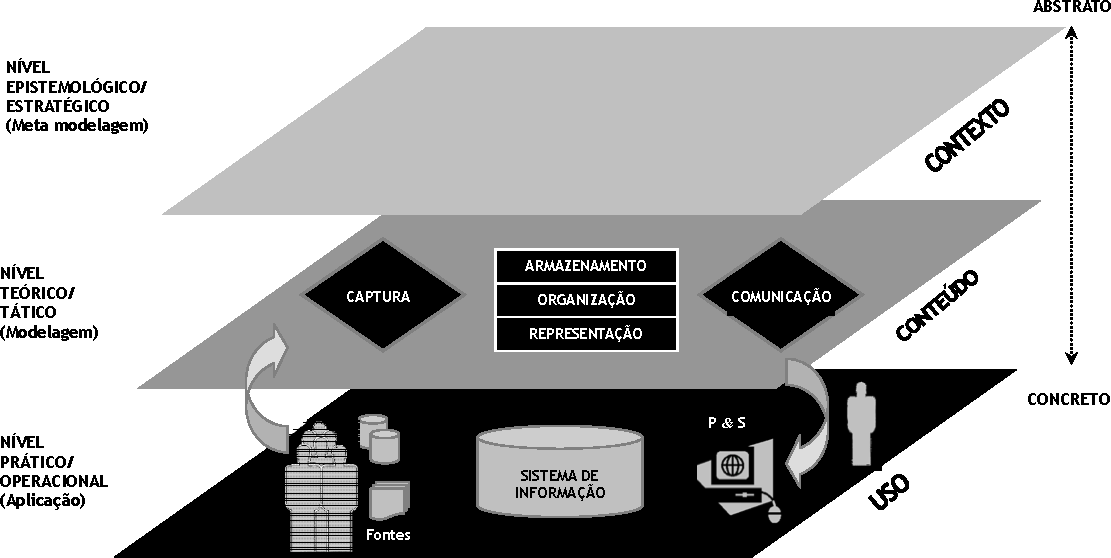
\includegraphics[scale=0.8]{imagens/fig_modeloAIMacedo.pdf}
  	\caption{\label{fig_m3hier}Metodologia de Meta-Modelagem (M{$^3$}):
  	hierarquia de sistemas de investigação}
  	\caption*{Fonte: \citeonline[p. 74]{van86}} 
\end{center} 
\end{figure}

A \autoref{tab-nivinv}\ldots

\begin{table}[htb]
\footnotesize
\caption[Níveis de investigação]{\footnotesize{Níveis de investigação.
\cite{van86}}}
\label{tab-nivinv}
\begin{tabular}{p{2.6cm}|p{6.0cm}|p{2.25cm}|p{3.40cm}}
  %\hline
   \textbf{Nível de Investigação} & \textbf{Insumos}  & \textbf{Sistemas de Investigação}  & \textbf{Produtos}  \\
    \hline
    Meta-nível & Filosofia da Ciência  & Epistemologia & Paradigma  \\
    \hline
    Nível do objeto & Paradigmas do metanível e evidências do nível inferior &
    Ciência  & Teorias e modelos \\
    \hline
    Nível inferior & Modelos e métodos do nível do objeto e problemas do nível inferior & Prática & Solução de problemas  \\
   % \hline
\end{tabular}
\end{table}


%---------------------------------------------------------------------
\section{Fontes de pesquisa} \label{metodologiaFontes}
%---------------------------------------------------------------------

A revisão da literatura foi realizada principalmente nas --- mas não limitada às
--- fontes seguintes:

\textbf{Bancos de Testes e Dissertações}

\begin{list}{--}{\parsep0.0cm\leftmargin2.0cm}
  \item Banco de Teses da CAPES (\url{http://www.capes.gov.br/servicos/banco-de-teses/});
  \item Banco de Teses e Dissertações da UnB (\url{http://bce.unb.br/});
\end{list}

\textbf{Bases de Dados}

\begin{list}{--}{\parsep0.0cm\leftmargin2.0cm}
  \item ACM Digital Library (\url{http://dl.acm.org/});
  \item Periódicos CAPES (\url{http://www.periodicos.capes.gov.br/})
  \item ProQuest (\url{http://search.proquest.com/})
  \item School of Information (\url{http://www.ischool.utexas.edu/});
  \item Web of Knowledge (\url{http://wok.mimas.ac.uk/});
  \item \ldots
\end{list}

\textbf{Periódicos}

\begin{list}{--}{\parsep0.0cm\leftmargin2.0cm}
  \item Ciência da Informação (IBICT);
  \item Journal of the American Society for Information Science and Technology
  (JA-SIST);
\end{list}

%---------------------------------------------------------------------
%---------------------------------------------------------------------
\subsection{Bibliometria}\label{metodologiaBibliometria}
%---------------------------------------------------------------------

A \autoref{tab_bibliometria_termosInformationConfig} contém dados bibliométricos
de pesquisas de termos chaves em algumas das bases de dados listadas na
\autoref{metodologiaFontes}\ldots

% EXEMPLO DE LONG TABLE
% INFORMATION e CONFIGURATION - Tabela principal de consultas de
\begin{center}
\footnotesize{
\begin{ThreePartTable}

\begin{longtable}{p{7.2cm}|p{6.3cm}|p{1.8cm}}

\caption[Resultados obtidos na consulta de termos ``configuration'' e
``information'' em bases de dados em 29.1.2012.]{\footnotesize{Resultados obtidos
na consulta de termos ``configuration'' e ``information'' em bases de dados.
Consultas realizadas em 29.1.2012. Período pesquisado: todos disponíveis nas
bases.}}
\label{tab_bibliometria_termosInformationConfig}
\\

%This is the header for the first page of the table...
\hline 
\textbf{Base de dados}	& \textbf{Termos e critérios} & \textbf{Resultados} \\
\hline 
%\endfirsthead
\endhead

%This is the footer for all pages except the last page of the table...
  \multicolumn{3}{r}{{Continua\ldots\ldots}} \\
\endfoot

%This is the footer for the last page of the table...
\hline \hline
\endlastfoot

%Now the data...

    % ``information configuration''
	\multirow{2}{*}{Academic Search Premier - ASP (EBSCO)}\tnote{a}
	& Titulo=(``information configuration'')
	& 1\tnote{b}
	\\
	& Titulo=(``configuration of information'')
	& 1\tnote{e}	
	\\ \hline	

	\multirow{2}{*}{Cambridge Journals Online}\tnote{a}
	& Titulo=(``information configuration'')
	& 0
	\\
	& Titulo=(``configuration of information'')
	& 0
	\\ \hline	

	\multirow{2}{*}{Highwire Press}\tnote{a}
	& Titulo=(``information configuration'')
	& 0
	\\
	& Titulo=(``configuration of information'')
	& 0
	\\ \hline	

	\multirow{2}{*}{Nature (NPG)}\tnote{a}
	& Titulo=(``information configuration'')
	& 0
	\\
	& Titulo=(``configuration of information'')
	& 0
	\\ \hline	

	\multirow{2}{*}{Oxford Journals (Oxford University Press)}\tnote{a}
	& Titulo=(``information configuration'')
	& 0
	\\
	& Titulo=(``configuration of information'')
	& 0
	\\ \hline	

	\multirow{3}{*}{SciELO.ORG}\tnote{a}
	& Titulo=(``information configuration'')
	& 0
	\\
	& Titulo=(``configuration of information'')
	& 0
	\\
	& Title: ``configuração da informação''
	& 0
	\\ \hline	

	\multirow{2}{*}{Science (AAAS)}\tnote{a}
	& Titulo=(``information configuration'')
	& 0
	\\
	& Titulo=(``configuration of information'')
	& 0
	\\ \hline	

	\multirow{2}{*}{ScienceDirect (Elsevier)}\tnote{a}
	& Titulo=(``information configuration'')
	& 0
	\\
	& Titulo=(``configuration of information'')
	& 0
	\\ \hline	

	\multirow{2}{*}{SpringerLink (MetaPress)}\tnote{a}
	& Titulo=(``information configuration'')
	& 0
	\\
	& Titulo=(``configuration of information'')
	& 0
	\\ \hline	

	\multirow{2}{*}{E-LIS}
	& Title: ``information configuration''
	& 2\tnote{c}
	\\
	& Title: ``configuration of information''
	& 1\tnote{d}
	\\ \hline	

	\multirow{2}{*}{Web of Knowledge}
	& Title: ``information configuration''
	& 0
	\\
	& Title: ``configuration of information''
	& 0
	\\ \hline	
	
\end{longtable}

	\begin{tablenotes}
		\item [a] Base de Periódicos CAPES.
		\item [b] O único texto obtido \ldots
		\item [c] Os textos recuperados \cite{hammer2005} e \cite{apps2001} se
		referem, respectivamente, a um manual de uso de uma ferramenta de
		gerenciamento de informação para bibliotecários e a um serviço baseado em Dublincore.
		\item [d] O único texto obtido \ldots
		\item [e] O único texto obtido \ldots

	\end{tablenotes}
	
\end{ThreePartTable}
}
\end{center}


% Figura - Web of Science 1 - Detalhamento
\begin{figure}[htb]
\begin{center}
  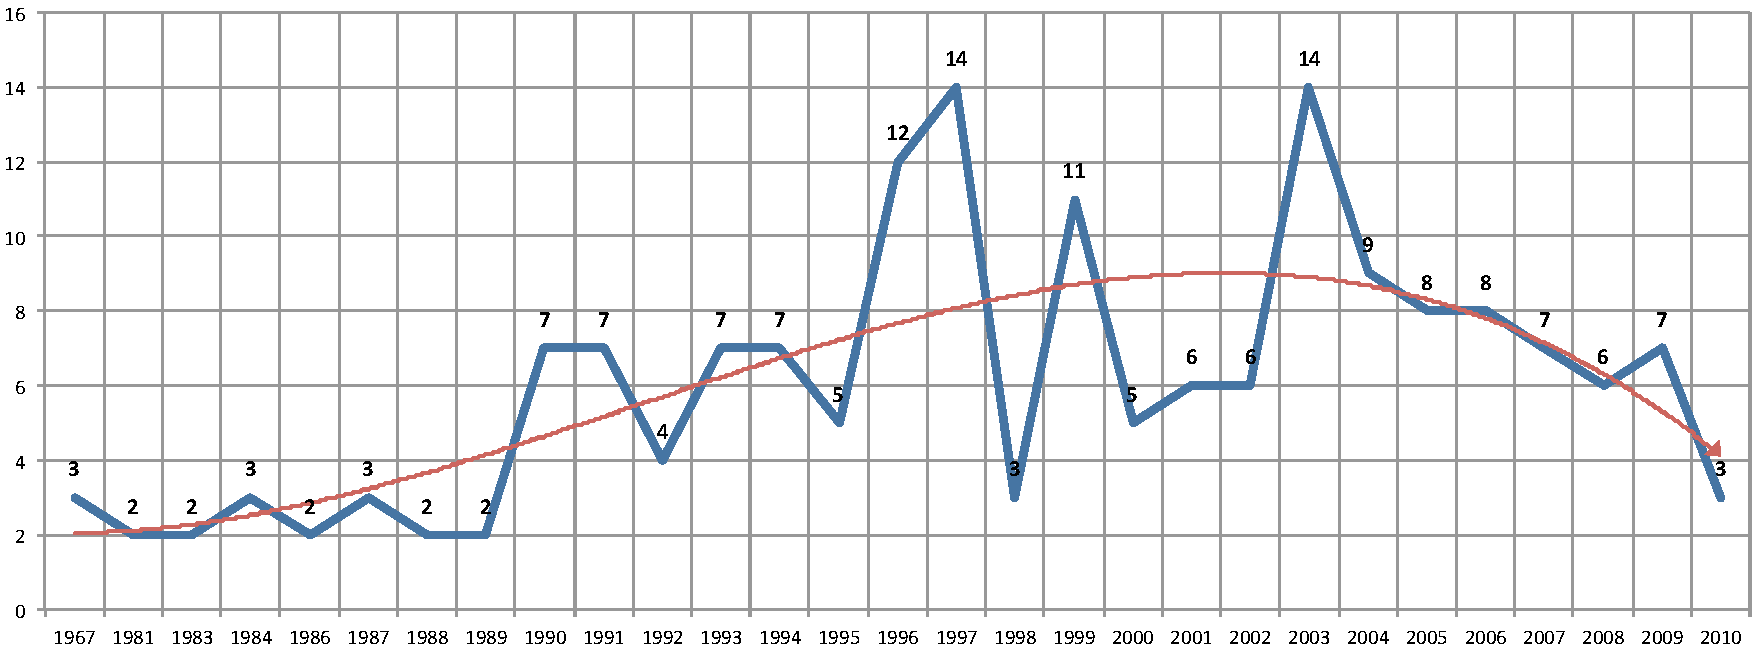
\includegraphics[scale=0.55]{imagens/bibliometriaWebOfScience1.pdf}
  \caption{\label{fig_biblioWebOfScience1}Bibliometria - Web of Science -
  Detalhamento da consulta - Critério: Title=(``configuration management'').}
  \caption*{Fonte: autores}
\end{center}
\end{figure}


%---------------------------------------------------------------------


%---------------------------------------------------------------------
% SEGUNDA PARTE DO TRABALHO
% revisao da literatura - fundamentos
%---------------------------------------------------------------------

\part{Revisão de Literatura e Fundamentos}

\chapter*{Prólogo}

Nesta parte do texto são expostos\ldots

Cada um desses tópicos são encontrados nos capítulos da seguinte maneira:

\begin{list}{--}{\parsep0.0cm\leftmargin2.0cm} 

  \item \textbf{\autoref{resultadoAIRei} - \nameref{resultadoAIRei}}: aborda\ldots

  \item \ldots 
  
\end{list}

%---------------------------------------------------------------------
% CAPITULOS
%---------------------------------------------------------------------

%------------------------------------------------
\chapter{Revisão 1} \label{cap_ai}
%------------------------------------------------

%------------------------------------------------
\section{Introdução}
%------------------------------------------------

Neste capítulo \ldots


%------------------------------------------------
\section{Seção sobre isso}
%------------------------------------------------

%------------------------------------------------
\section{Seção sobre aquilo}
%------------------------------------------------

Neste capítulo \ldots

%------------------------------------------------
\section{Seção sobre queijo}
%------------------------------------------------

Neste capítulo \ldots

%------------------------------------------------
\section{Seção sobre pamonha}
%------------------------------------------------

Neste capítulo \ldots

%------------------------------------------------
\section{Seção sobre milho cozinho com sal e águla}
%------------------------------------------------

Neste capítulo \ldots

%------------------------------------------------
\section{Conclusão}
%------------------------------------------------

Neste capítulo \ldots




%---------------------------------------------------------------------
% TERCEIRA PARTE DO TRABALHO
% resultados
%---------------------------------------------------------------------

\part{Resultados}

%---------------------------------------------------------------------
% CAPITULOS
%---------------------------------------------------------------------

\chapter{Resultado 1}
\label{cap_resultadoAI}

%-----------------------------
\section{Introdução}
%-----------------------------

Este capítulo apresenta \ldots

A \autoref{resultadoAIRei} apresenta\ldots

%-----------------------------
\section{Título AI e o rei}\label{resultadoAIRei}
%-----------------------------



%---------------------------------------------------------------------
% CONSIDERACOES FINAIS
%---------------------------------------------------------------------

%finaliza a parte
\bookmarksetup{startatroot}% this is it
\addtocontents{toc}{\bigskip}% perhaps as well

%Considerações finais

%~~~~~~~~~~~~~~~~~~~~~~~~~~~~~~~~~~~~~~~~~~~~~~~~~~~~~~~~~~~~~~~~~~~~~
%
%    File       : conclusão
%    Type       : TeX
%    Date       : terça-feira, março 01, 2011 at 10:57
%
%    Content 	: Considerações gerais sobre a pesquisa e o resultado
%~~~~~~~~~~~~~~~~~~~~~~~~~~~~~~~~~~~~~~~~~~~~~~~~~~~~~~~~~~~~~~~~~~~~~

%---------------------------------------------------------------------
\chapter{Considerações finais}\label{cap_conclusao}
%---------------------------------------------------------------------

Este trabalho\ldots

%---------------------------------------------------------------------
\section{Contribuições e alcance dos objetivos}
\label{conclusao_contribuicoes}
%---------------------------------------------------------------------

Nesta seção estão listadas, na ordem em que apareceram no texto, algumas das
contribuições mais importantes desta pesquisa.

\begin{list}{--}{\leftmargin2cm\parsep0.2cm}

    \item Derivações jklfgjklfjd;

    \item Modelos e Métodos para klfkjfls;d;

    \item Estudos de casos jffdjsfdsj;

    \item Elaboração de modelos de operacionalização jjfdjskjk;

    \item Avaliação de impacto jkflsdl; e,

    \item Modelo de comunicação jfdjfsdjklj.

\end{list}

%---------------------------------------------------------------------
\section{Possibilidades de pesquisas futuras}\label{conclusaoTrabalhosFuturos}
%---------------------------------------------------------------------

\begin{list}{--}{\leftmargin2cm\parsep0.2cm}

    \item Derivações jklfgjklfjd;

    \item Modelos e Métodos para klfkjfls;d;

    \item Estudos de casos jffdjsfdsj;

    \item Elaboração de modelos de operacionalização jjfdjskjk;

    \item Avalição de impacto jkflsdl; e,

    \item Modelo de comunicação jfdjfsdjklj.

\end{list}

%~~~~~~~~~~~~~~~~~~~~~~~~~~~~~~~~~~~~~~~~~~~~~~~~~~~~~~~~~~~~~~~~~~~~~
%	ELEMENTOS PÓS-TEXTUAIS
%~~~~~~~~~~~~~~~~~~~~~~~~~~~~~~~~~~~~~~~~~~~~~~~~~~~~~~~~~~~~~~~~~~~~~


%---------------------------------------------------------------------
% REFERENCIAS - bibliografia
%---------------------------------------------------------------------
\bibliography{bib/references}

% ---------------------------------------------------------------------
% GLOSSÁRIO
% ---------------------------------------------------------------------
% Não utilize ponto (.) no final das frases. Ele é adicionado automaticamente
%
% Para compilar o glossario, digite no prompt:
%    makeglossaries main.tex
% Recompile o projeto
% 

\newglossaryentry{palavraChave1}{ 
	name={nome no singular},
	plural={nome no plural},
	description={conjunto de \glspl{produto} ou de \glspl{itemConfiguracao} que
	juntos possuem uma fronteira bem definida de tal forma que se tornam um item
	individual de configuração. São partes de produtos finais ou de
	outros componentes} }

\newglossaryentry{produto}{ 
	name={produto},
	plural={produtos},
	description={produto é o resultado de um processo} }

\newglossaryentry{itemConfiguracao}{ 
	name={item de configuração},
	plural={itens de configuração},
	description={conjunto de \glspl{produto} no plural ou de \gls{produto} no
	singular} }

\glsaddall
\renewcommand{\glossaryname}{Glossário} 
\renewcommand{\glossarypreamble}{Este glossário\ldots}

%Traduções para o ambiente glossaries
\providetranslation{Glossary}{Glossário}
\providetranslation{Acronyms}{Siglas}
\providetranslation{Notation (glossaries)}{Notação}
\providetranslation{Description (glossaries)}{Descrição} 
\providetranslation{Symbol (glossaries)}{Síimbolo}
\providetranslation{Page List (glossaries)}{Lista de Páginas} 
\providetranslation{Symbols (glossaries)}{Símbolos}
\providetranslation{Numbers (glossaries)}{Números}

\glossarystyle{altlisthypergroup}
\printglossaries

%---------------------------------------------------------------------
% APÊNDICES
%---------------------------------------------------------------------
\apendice

\chapter{Apêndice AI}
\label{apendiceAI}

Texto

%---------------------------------------------------------------------
% ANEXOS
%---------------------------------------------------------------------
\anexo

\chapter{Anexo AI}
\label{anexoAI}

Este anexo contém\ldots

%---------------------------------------------------------------------
% INDICE REMISSIVO
%---------------------------------------------------------------------


\cleardoublepage
\phantomsection 
\addcontentsline{toc}{chapter}{\indexname}
\ProximoForaDoSumario
\printindex

%---------------------------------------------------------------------

\end{sloppypar}											% Fecha ambiente/container

\end{document}											% Fecha a classe document

%~~~~~~~~~~~~~~~~~~~~~~~~~~~~~~~~~~~~~~~~~~~~~~~~~~~~~~~~~~~~~~~~~~~~~